\section{Modellierung der Systemdynamik}
In dem folgenden Abschnitt werden die Bewegungsgleichungen mit Hilfe des Lagrange Formalismus hergeleitet. Aus diesen Gleichung kann im Anschluss eine Zustandsraumdarstellung aufgestellt werden, welche als Grundlage für den Reglerentwurf dient.

\begin{figure}[h]
\centering
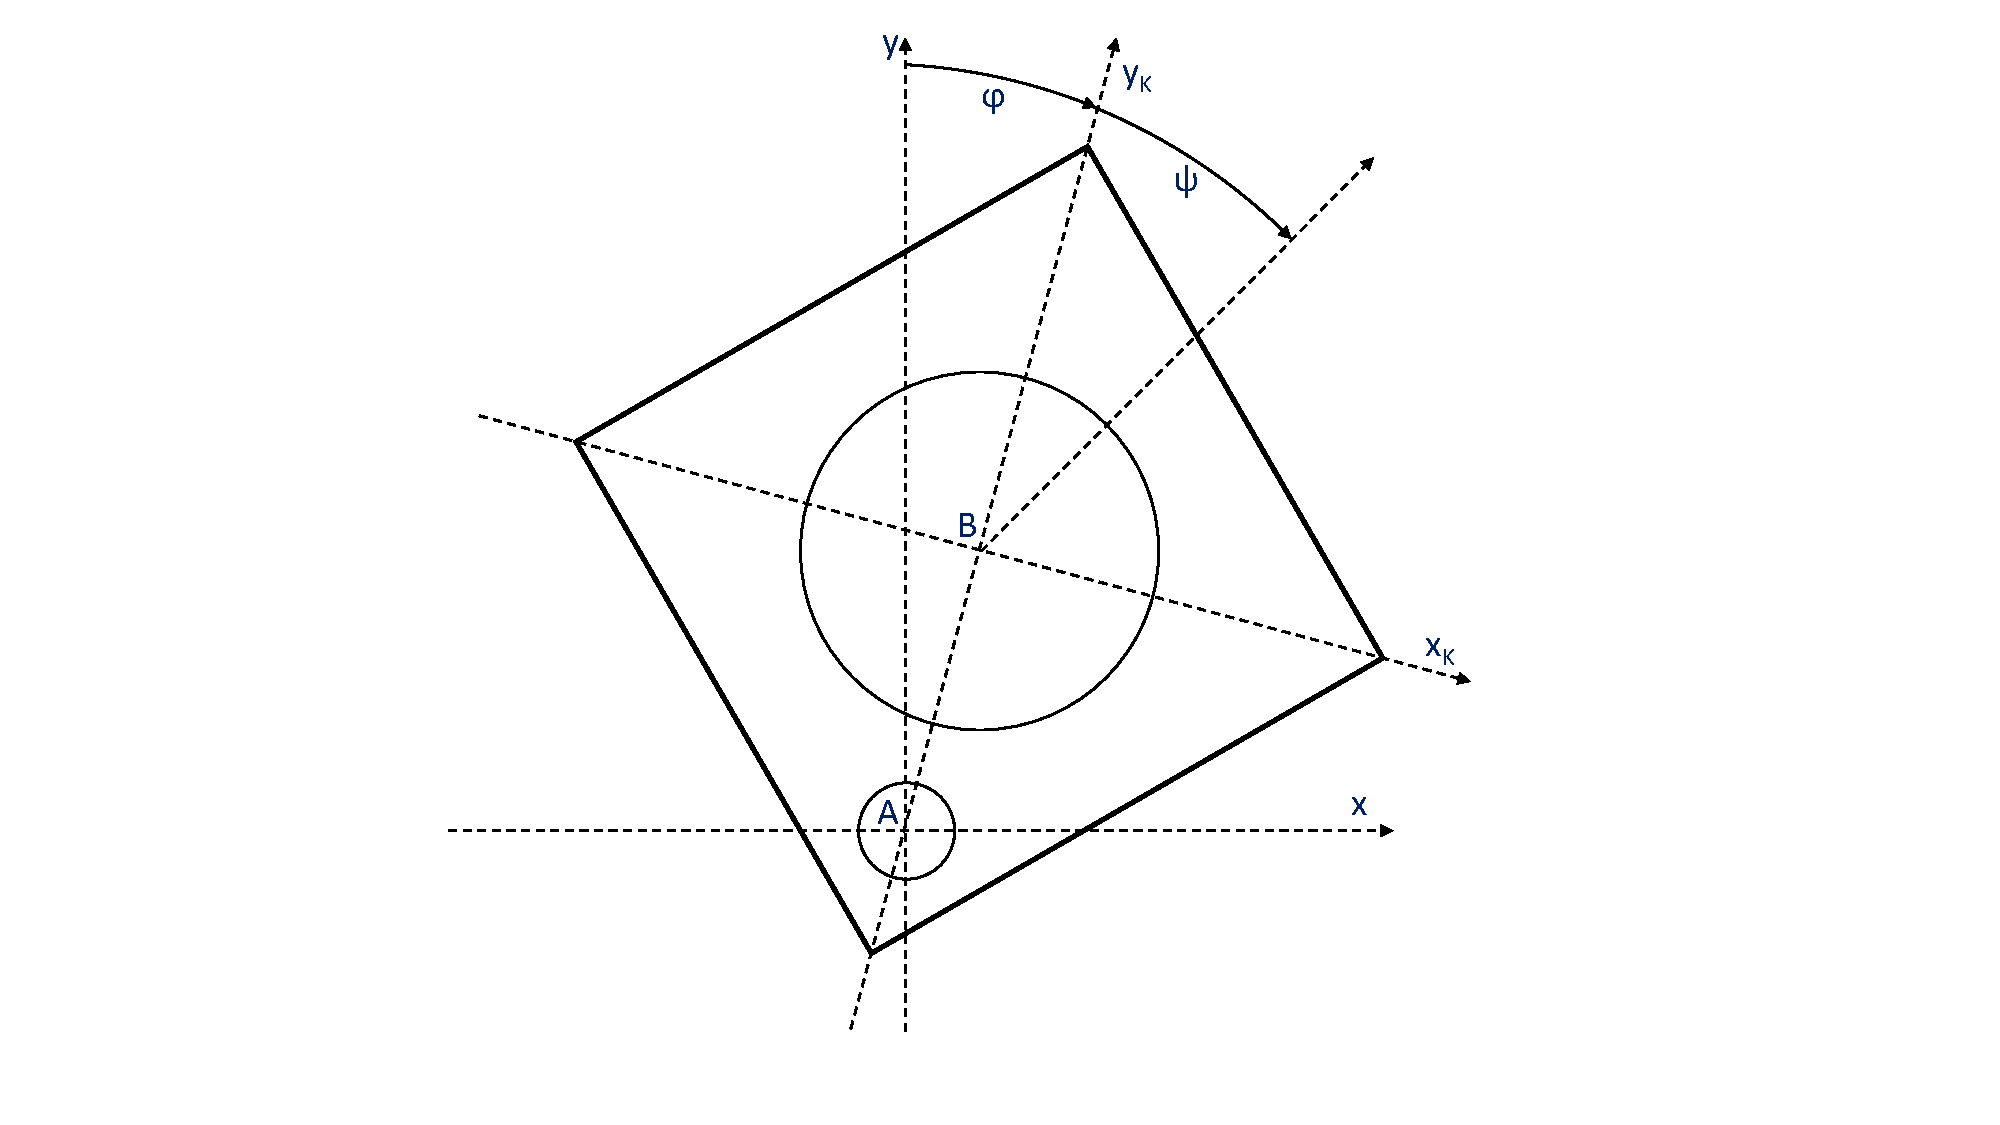
\includegraphics[width=\linewidth]{MechZeichnung1D}
\caption{Mechanischer Aufbau, Quelle: eigene Darstellung}
\end{figure}

Der Prototyp besteht aus einem starren Körper der in $A$ auf einer Achse gelagert ist. In $B$ ist eine Schwungmasse über einen Motor mit dem Körper verbunden. Somit verfügt das Gesamtsystem über zwei Freiheitsgrade, welche durch die generalisierten Koordinaten 

\begin{equation}
q_1 = \varphi \hspace{35pt} q_2 = \psi
\end{equation}

beschrieben werden. Der Winkel $\varphi$ wird von den Achsen $y$ und $y_K$ eingeschlossen. Der Winkel beschreibt die rotatorische Verschiebung der Schwungmasse zu dem Körper. Die folgenden Größen beschreiben die weiteren physikalischen Gegebenheiten des Systems.\newline

\begin{table}[h]
\centering
\begin{tabular}{ll}
	$q_1 = \varphi$ & Ausfallwinkel des Körpers \\
	$q_2 = \psi$ & Winkel zwischen Schwungmasse und Körper \\
	$A$ & Drehpunkt des Körpers \\
	$B$ & Drehpunkt des Schwungrades \\
	$l_{AB}$ & Abstand zwischen $A$ und $B$ \\
	$l_{AC}$ & Abstand zwischen $A$ und dem Schwerpunkt des Körpers \\
	$m_K$ & Masse des Körpers \\
	$m_R$ & Masse des Schwungrades \\
	$J^A_K$ & Massenträgheitsmoment des Körper um $A$ \\
	$J^B_R$ & Massenträgheitsmoment der Schwungmasse um $B$ \\
	$C_{\varphi}$ & Dynamischer Reibkoeffizient des Körpers in $A$ \\
	$C_{\psi}$ & Dynamischer Reibkoeffizient des Schwungrades in $B$ \\
	$T_M$ & Drehmoment des Motor
\end{tabular}
\end{table}

\newpage
Um die Bewegungsgleichungen des Systems zu ermitteln wird der Lagrange Formalismus verwendet. Dieser basiert auf der Lagrange-Funktion $L$, welche die Differenz der kinetischen Energie $T$ und der potenziellen Energie $V$ des Systems beschreibt.

\begin{equation}
T = \frac{1}{2}[(J^A_K + m_R \cdot {l_{AB}}^2) {\dot{\varphi}}^2 + J^R_B(\dot{\varphi}+\dot{\psi})^2]
\end{equation}
\begin{equation}
V = g(m_R \cdot l_{AB} + m_K \cdot l_{AC})cos(\varphi)
\end{equation}
\begin{equation}
L = T - V = \frac{1}{2}[(J^A_K + m_R \cdot {l_{AB}}^2) {\dot{\varphi}}^2 + J^R_B(\dot{\varphi}+\dot{\psi})^2] - g(m_R \cdot l_{AB} + m_K \cdot l_{AC})cos(\varphi)
\end{equation}

Das von dem Motor verursachte Drehmoment $T_M$ verrichtet die virtuelle Arbeite $\delta W_M$. Aus diesem können die generalisierten Kraftkomponenten $Q_{\varphi}$ und $Q_{\psi}$ abgeleitet werden.

\begin{equation}
\delta W_M = T_M \cdot \delta \psi
\end{equation}
\begin{equation}
Q_{\varphi} = T_M \cdot \frac{\partial \psi}{\partial \varphi} = 0
\end{equation}
\begin{equation}
Q_{\psi} = T_M \cdot \frac{\partial \psi}{\partial \psi} = T_M
\end{equation}

Durch die Reibung in den Lagerungen bei $A$ und $B$ geht Energie in dem System verloren. Diese Verlustleistung kann mit den Rayleigh'schen Dissipationsfunktionen $D_{\varphi}$ und $D_{\psi}$ beschrieben werden.

\begin{equation}
D_{\varphi} = \frac{1}{2}C_{\varphi} \cdot {\dot{\varphi}}^2
\end{equation}
\begin{equation}
D_{\psi} = \frac{1}{2}C_{\psi} \cdot {\dot{\psi}}^2
\end{equation}
\begin{equation}
D = D_{\varphi} + D_{\psi} = \frac{1}{2}C_{\varphi} \cdot {\dot{\varphi}}^2 + \frac{1}{2}C_{\psi} \cdot {\dot{\psi}}^2
\end{equation}

Bei dem Prototyp handelt es sich um ein nicht konservatives System, da einerseits durch die Reibung mechanische Energie verloren geht. Andererseits erhöht das Motormoment die mechanische Gesamtenergie des Systems. Da die beiden generalisierten Koordinaten $\varphi$ und $\psi$ voneinander unabhängig sind können aus dem d'Alembert'schen Prinzip zwei Bewegungsgleichungen abgeleitet werden.

\begin{equation}
\frac{d}{dt}\frac{\partial L}{\partial \dot{q}_i}-\frac{\partial L}{\partial q_i} + \frac{\partial D}{\partial \dot{q}_i} = Q_i
\end{equation}
\begin{equation}
\frac{d}{dt}\frac{\partial L}{\partial \dot{\varphi}}-\frac{\partial L}{\partial \varphi} + \frac{\partial D}{\partial \dot{\varphi}} = Q_{\varphi} 
\end{equation}
\begin{equation}
\label{LG_phi_equation}
(J^A_K + J^R_B + m_R \cdot l_{AB})\ddot{\varphi} + J^R_B \cdot \ddot{\psi} - g(m_R \cdot l_{AB} + m_K \cdot l_{AC})sin(\varphi) + C_{\psi} \cdot \dot{\psi} = 0
\end{equation}
\begin{equation}
\frac{d}{dt}\frac{\partial L}{\partial \dot{\psi}}-\frac{\partial L}{\partial \psi} + \frac{\partial D}{\partial \dot{\psi}} = Q_{\psi} 
\end{equation}
\begin{equation}
\label{LG_psi_euqation}
J^R_B \cdot \ddot{\psi} = T_M - C_{\psi} \cdot \dot{\psi} - J^R_B \cdot \ddot{\varphi}
\end{equation}

Durch Einsetzen von (\ref{LG_psi_euqation}) in (\ref{LG_phi_equation}) ergibt sich die folgende Bewegungsgleichung für die Würfelseite.

\begin{equation}
\label{BG_phi_quation}
\ddot{\varphi} = \frac{g(m_R \cdot l_{AB} + m_K \cdot l_{AC})sin(\varphi) - C_{\varphi} \cdot \dot{\varphi} + C_{\psi} \cdot \dot{\psi} - T_M}{J^A_K + m_R \cdot l_{AB}}
\end{equation}

Die Bewegungsgleichung für die Schwungmasse ergibt sich durch Einsetzen von (\ref{BG_phi_quation}) in (\ref{LG_psi_euqation}).

\begin{equation}
\label{BG_psi_equation}
\ddot{\psi} = \frac{(J^A_K + m_R \cdot l_{AB} + J^R_B)(T_M - C_{\psi} \cdot \dot{\psi})}{(J^A_K + m_R \cdot {l_{AB}}^2)J^R_B} + \frac{C_{\varphi} \cdot \dot{\varphi} - g(m_R \cdot l_{AB} + m_K \cdot l_{AC})sin(\varphi)}{J^A_K + m_R \cdot {l_{AB}}^2}
\end{equation}